\documentclass[tikz,border=2pt]{standalone}
\usepackage{amsmath}
\usepackage{pgfplots}
\pgfplotsset{compat=1.18}

\begin{document}
% A series of functions Σ f_n is the limit of the partial-sum functions s_N = f_1 + ... + f_N:
% here f_n(x) = sin(nx)/n^2, with s_1, s_2, s_4 and the limit s.
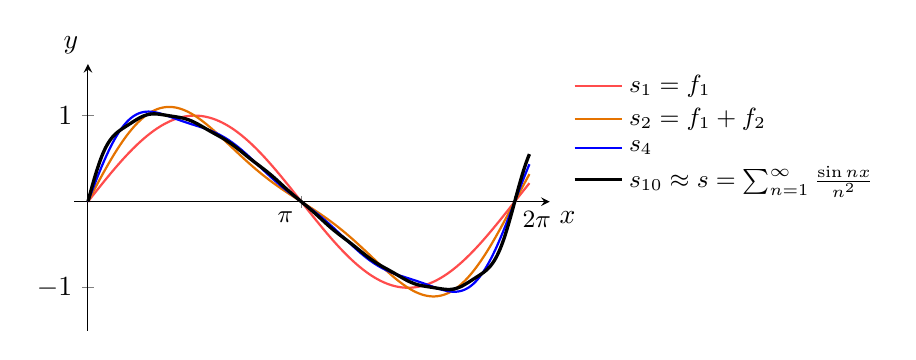
\begin{tikzpicture}
	\begin{axis}[
		axis lines=middle,
		xmin=-0.2, xmax=6.8,
		ymin=-1.5, ymax=1.6,
		xtick={3.1416,6.2832}, xticklabels={,}, ytick={-1,1},
		xlabel={$x$}, ylabel={$y$},
		xlabel style={below right}, ylabel style={above left},
		samples=300, smooth, clip=false,
		width=7.62cm, height=4.97cm,
		legend pos=outer north east, legend style={draw=none, fill=none, font=\small}, legend cell align=left
		]
		\addplot[thick, red!70, domain=0:6.5] {sin(deg(x))};
		\addlegendentry{$s_1=f_1$}
		\addplot[thick, orange!90!black, domain=0:6.5] {sin(deg(x))+sin(deg(2*x))/4};
		\addlegendentry{$s_2=f_1+f_2$}
		\addplot[thick, blue, domain=0:6.5] {sin(deg(x))+sin(deg(2*x))/4+sin(deg(3*x))/9+sin(deg(4*x))/16};
		\addlegendentry{$s_4$}
		\addplot[very thick, black, domain=0:6.5] {sin(deg(x))+sin(deg(2*x))/4+sin(deg(3*x))/9+sin(deg(4*x))/16+sin(deg(5*x))/25+sin(deg(6*x))/36+sin(deg(7*x))/49+sin(deg(8*x))/64+sin(deg(9*x))/81+sin(deg(10*x))/100};
		\addlegendentry{$s_{10}\approx s=\sum_{n=1}^{\infty}\frac{\sin nx}{n^2}$}
		\node[anchor=north east, font=\small, inner sep=1.5pt] at (axis cs:3.09,-0.06) {$\pi$};
		\node[anchor=north west, font=\small, inner sep=1.5pt] at (axis cs:6.33,-0.06) {$2\pi$};
	\end{axis}
\end{tikzpicture}
\end{document}
